\chapter{Постановка задачи}
\section{Вводные}
В компании N планируется разработать модель машинного обучения, которая сможет определять структуру документа (вложенные списки) и внедрить в бизнес-процесс по анализу документов в предприятии K.

Структура документа --- это преобразование документа в древовидную структуру, каждый узел которой имеет какое-либо логическое определение или объяснение.

\section{Развитие}

Автоматизация полного цикла внедрения ML-сервиса:
\begin{itemize}
\item Разметка данных.
\item Обучение модели.
\item Применение модели.
\item Доразметка данных или активное обучение.
\item Дообучение модели.
\end{itemize}

\section{Техническое задание}
\begin{enumerate}
\item Должна быть разработана схема взаимодействия пользователя с системой.
\item Должна быть разработана схема взаимодействия (API) между компонентами ML-сервиса.
\item Должна быть разработана модель, которая принимает на вход текст документа и возвращает структуру документа.
\item Должен быть разработан отчет о ходе работ. Отчет должен включать следующую информацию:
  \begin{enumerate}
  \item Описание данных (определение типов данных, используемых в сервисе, и их структура).
  \item Эксперименты с моделями (описание экспериментов, проведенных при разработке модели, включая выбор датасетов, параметров обучения и результаты).
  \end{enumerate}
\end{enumerate}
\chapter{Ход работы}
\section{Описание данных}
Предоставленные данные --- нормативно-правовые акты из Единого реестра образовательных документов (ЕРОТ), 2000 документов в формате Portable Document Format. Несмотря на применение обработки естественного языка в широком круге задач при обработке PDF, большинство алгоритмов, использующих NLP, подразумевают использование «чистых данных». Для успешного определения целевой информации необходимо выявить иерархическую структуру для удаления незначительной информации из документа, к примеру, номера страницы.

Мы придерживаемся метода, разработанного Yuta Koreeda и Christofer D. Manning в статье «Захват логической структуры визуально структурированных документов с помощью мультимодального анализатора переходов» (Capturing Logical Structure of Visually Structured Documents with Multimodal Transition Parser). Этот метод позволяет практически не использовать разметку и оперировать высокоуровневыми признаками: визуальными (отступами, интерльяжем) и текстовыми (пунктуацией, номерами в оглавлении).

На вход сервиса поступает PDF-файл для анализа, пользователь получает структуру документа в виде дерева в формате JSON.

Для каждого документа выполняются следующие шаги:

\begin{enumerate}
\item Создается пустой словарь \texttt{spans} для хранения информации о блоках текста.
\item Для каждого блока текста в документе выполняются следующие действия:
  \begin{itemize}
  \item Строится матрица иерархии \texttt{(m)} с использованием функции \texttt{create\_hierarchy\_matrix}.
  \item Для каждого индекса блока текста проверяются отношения с другими блоками текста.
  \item Информация о каждом блоке текста добавляется в словарь \textt{spans}.
  \end{itemize}
\item Формируется путь вывода \textt{(out\_path)} для каждого документа и сохраняется в формате JSON с использованием json.dump.
\end{enumerate}

\section{Описание модели}
\subsection{Гипотезы}
В ходе работ были предложены три основные методологии выполнения работы:
\begin{enumerate}
\item Использование больших языковых моделей для выявления структуры. Достоинства такого метода: отстутствие необходимости разметки данных, возможность вывода в формате, нужном пользователю, способны улавливать сложный контекст и взаимосвязь между разными частями документа, автоматически извлекать признаки и паттерны. Недостатки такого метода: требования к вычислительным ресурсам (как для обучения, так и для инференса), неясность интерпретации принятия решения моделью, возможность «галлюцинаций» в выводе, сложность применения в доменной области из-за чувствительного характера данных.
\item Использование XML-структур и заголовков для выявления структуры документа. Достоинства такого метода: XML обеспечивает явную иерархию элементов, документы с явной структурой могут быть легко интерпретированы и поняты человеком без необходимости автоматического анализа, требуется малое количество вычислительных ресурсов. Недостатки такого метода: XML может не явно представлять некоторые отношения между различными частями документа, XML-структуры могут оказаться не достаточно гибкими для представления динамичных или сложных структур, в некоторых случаях автоматический анализ XML может требовать дополнительной обработки для выделения семантической структуры.
\item Использование ручных признаков и классификатора на основе машинного обучения. Достоинства:
  \begin{enumerate}
  \item Возможность включения в модель различных признаков, таких как визуальные, текстовые и семантические, что может улучшить способность модели к анализу контента.
  \item Может быть эффективным в случаях, когда у нас есть ограниченное количество обучающих данных, что важно в юридической области, где многие данные являются закрытыми.
  \item Ручные признаки обычно более легко интерпретируются, что облегчает понимание принимаемых моделью решений.
  \item Обучение модели на основе ручных признаков и классификатора может быть более быстрым и требовать меньше вычислительных ресурсов по сравнению с глубоким обучением.
   \end{enumerate}
  Недостатки:
  \begin{enumerate}
  \item Модели, основанные на ручных признаках, могут оказаться менее способными к автоматическому выявлению сложных и абстрактных паттернов, которые могли бы быть выучены глубокими нейронными сетями.
  \item Результаты сильно зависят от качества выбранных ручных признаков, и неправильный выбор может привести к ухудшению производительности.
  \item Модель, основанная на ручных признаках, может иметь ограниченные возможности в обобщении на новые и неизвестные сценарии, особенно если они сильно отличаются от обучающих данных.
  \item Сложность учета всех видов информации (визуальной, текстовой, семантической) может потребовать дополнительной тщательной обработки.
    \end{enumerate}
\end{enumerate}

Исходя из технического задания и доменной области был выбран вариант с использованием ручных признаков и классификатора на основе машинного обучения.

\subsection{Признаки, используемые моделью}

\begin{enumerate}
\item Отступы (вверх, вниз или одинаковые). Описывает отношение отступов между разными уровнями текстовых блоков (1-2, 2-3).
\item Отступы после отстутствия нумерации.
\item Центрированный. Описывает, является ли текст центрированным.
\item Разрыв строки перед правым краем.
\item Перенос на новую страницу.
\item В верхних 15\% страницы.    Описывает, находится ли блок в верхних 15\% страницы.
\item В нижних 15\% страницы.    Описывает, находится ли блок в нижних 15\% страницы.
\item Увеличенный межстрочный интервал. Описывает, есть ли увеличенный межстрочный интервал.
\item Выровнен по ширине с пробелами посередине. Описывает, выровнен ли текст по ширине с пробелами посередине.
\item Похожий текст в похожей позиции. Описывает наличие похожего текста в похожей позиции.
\item Выделение пробелами между символами. Описывает выделение пробелами между символами.
\item Выделение скобками. Описывает выделение текста скобками.
\end{enumerate}
\subsection{Эксперименты и метрики}
Конечная цель оценки эффективности системы заключается в том, чтобы понять, насколько хорошо она справляется с поставленной задачей. В данном случае система рассматривается как инструмент для извлечения информации из текста.

Первый набор метрик (IE-перспектива)
\begin{itemize}
\item Однозначный абзац: Метрика F1 оценивает, насколько успешно система идентифицирует пары блоков, находящихся в пределах одного абзаца.

\item Сиблинги: Аналогично, система оценивается на способность выявлять отношения сиблингов между блоками.

\item Отношения предок-потомок: Эта метрика оценивает способность системы выявлять отношения между блоками в иерархии предок-потомок.

\end{itemize}

Второй набор метрик (Предварительная обработка для NLP):
\begin{itemize}
\item Выделение границ абзацев: Эта метрика оценивает, насколько точно система определяет границы абзацев. Это важно для того, чтобы правильно передавать фрагменты текста в технологии обработки естественного языка (NLP).

\item Точность удаления мусора с опущенным абзацем: Метрика отражает эффективность системы в удалении блоков с опущенными изменениями.
\end{itemize}

Был использован Random Forest в качестве классификаторов для определения переходов и указателей. Random Forest подходит для работы с категориальными признаками, которые составляют основную часть наших характеристик (features).

Random Forest представляет собой ансамбль решающих деревьев, где каждое дерево принимает решение, и окончательный результат определяется голосованием или усреднением результатов отдельных деревьев. Этот метод хорошо подходит для задач классификации, особенно когда признаки могут быть категориальными.

В ходе экспериментов были проведены исследования важности каждой функции при использовании методов жадного прямого отбора (greedy forward selection) и жадного обратного исключения функций (greedy backward elimination). В ходе исследования было выяснено, что система балансированно использует визуальные и текстовые подсказки.

Некоторые параметры, такие как «Отступ», «Больший интерлиньяж» и «Иерархия нумерации (T1)», которые частично представляют собой целевые метрики, оказались высоко оцененными во многих случаях. В то же время другие параметры, такие как «Все заглавные буквы» и «Пунктуированные», также внесли значительный вклад в точность.
\section{Описание API}
Описание представлено на рисунке \ref{API0}.
API предназначено для обработки PDF-файлов и предсказания структуры документа с использованием библиотеки \texttt{pdf\_struct}.

\begin{enumerate}
    \item \textbf{Загрузка PDF-файла:} Пользователь отправляет POST-запрос на эндпоинт \texttt{/pdf}, включая PDF-файл в теле запроса. PDF-файл загружается с использованием \texttt{UploadFile} из FastAPI.
    
    \item \textbf{Сохранение PDF-файла:} Содержимое загруженного PDF-файла читается и сохраняется на сервере в директории \texttt{pdf} с использованием уникального имени файла.
    
    \item \textbf{Предсказание структуры PDF:} Загруженный PDF-файл передается в функцию \texttt{pdf\_struct.predict}, которая выполняет предсказание структуры документа. Параметры функции указывают формат вывода (\texttt{format='tree'}), путь к PDF-файлу (\texttt{in\_path=path\_to\_pdf\_file}), и используемую модель (\texttt{model='PDFContractEnFeatureExtractor'}).
    
    \item \textbf{Сохранение результата в текстовый файл:} Полученная структура документа преобразуется в строку и сохраняется в текстовом файле в директории \texttt{out}. Этот файл имеет уникальное имя, содержащее текущую дату и время.
    
    \item \textbf{Отправка результата пользователю:} Текстовый файл с результатами отправляется пользователю в качестве ответа на запрос с использованием \texttt{FileResponse}. Медиа-тип указывается как \texttt{"application/text"}, и имя файла также включает текущую дату и время.
    
    \item \textbf{Запуск и обслуживание сервера:} Если скрипт запускается напрямую (\texttt{if \_\_name\_\_ == "\_\_main\_\_":}), то сервер запускается с использованием \texttt{uvicorn} на localhost, порту 8000, с возможностью автоматической перезагрузки и тремя рабочими процессами.
\end{enumerate}
\begin{figure}
  \centering
  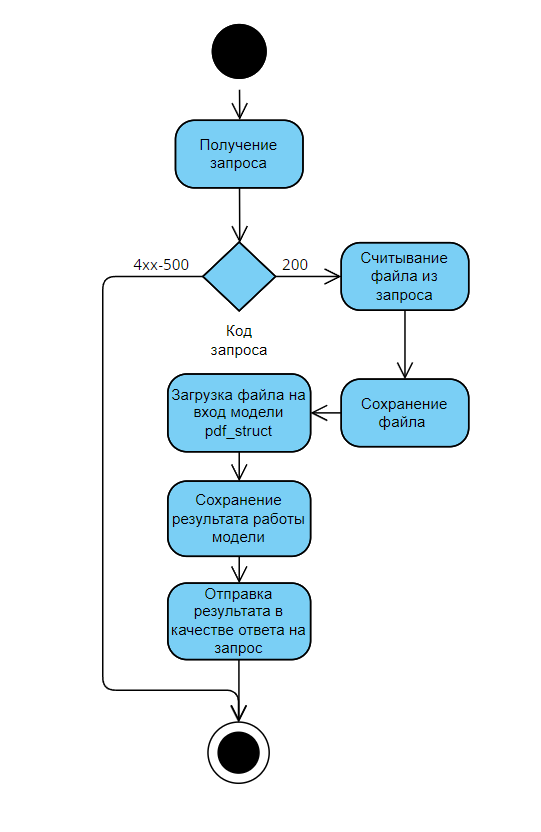
\includegraphics[width=0.5\linewidth]{API}
  \caption{Реализация API}
  \label{API0}
\end{figure}
\section{Описание взаимодействия пользователя с системой}
Код на Python использует библиотеку Aiogram для создания бота в Telegram.
Описание представлено на рисунке \ref{NIRR}.
\begin{figure}
  \centering
  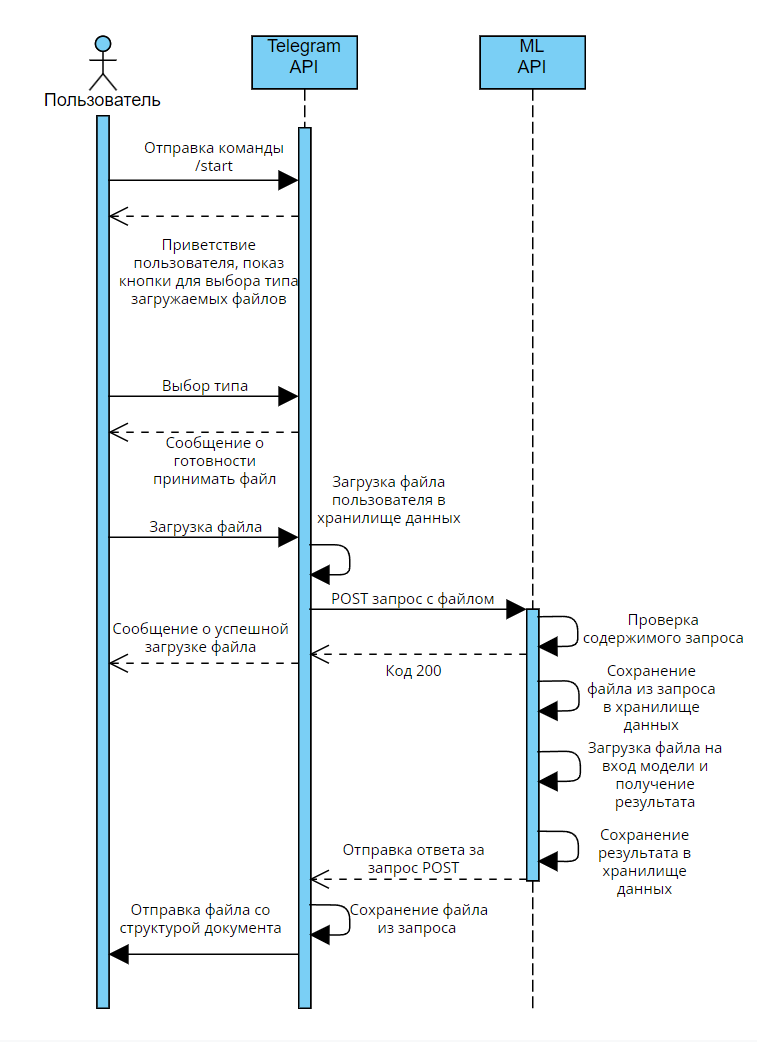
\includegraphics[width=\linewidth]{NIR}
  \caption{Описание взаимодействия пользователя с системой}
  \label{NIRR}
\end{figure}
\begin{enumerate}[label=\textbf{\arabic*.}]
    \item \textbf{Настройка команд бота:}
        Бот настроен на использование команд, таких как \texttt{/start} и \texttt{/help}. Команды устанавливаются с описанием, которое будет отображаться при запросе команд.

    \item \textbf{Обработчики сообщений:}
        \begin{enumerate}[label=\textbf{\alph*.}]
            \item \texttt{get\_start:} Этот обработчик вызывается при команде \texttt{/start} и приветствует пользователя, предлагая выбрать тип загружаемого файла.
            
            \item \texttt{start\_dow:} Обработчик, который запускается, когда пользователь выбирает загрузку PDF файла. Бот предлагает загрузить PDF файл.
            
            \item \texttt{dow\_file:} Обработчик загрузки файла. После того как пользователь загружает PDF файл, бот сохраняет его локально, отправляет на внешний сервер по адресу \url{http://localhost:8000/pdf}, получает ответ и отправляет результат пользователю.
        \end{enumerate}

    \item \textbf{Клавиатура для выбора действий:}
        Создается клавиатура с единственной кнопкой «Загрузить PDF». Эта клавиатура используется для удобного выбора действия при взаимодействии с ботом.

    \item \textbf{Основной блок кода:}
        В основном блоке кода создается экземпляр бота и диспетчера. Запускается функция \texttt{start()}, которая настраивает логирование, устанавливает команды бота и начинает прослушивание событий (\texttt{polling}).

    \item \textbf{Состояния для управления процессом загрузки:}
        В коде также определено состояние \texttt{DowPDF} с использованием \texttt{StatesGroup} из Aiogram. Это состояние используется для отслеживания этапа загрузки PDF файла.

    \item \textbf{Общий процесс работы бота:}
        Пользователь начинает с команды \texttt{/start}, затем выбирает загрузку PDF файла, загружает файл, и бот обрабатывает этот файл, отправляя его на внешний сервер и возвращая результат обратно пользователю.
\end{enumerate}
\chapter{Выводы}
В результате проведенных работ была разработана система с использованием машинного обучения для определения структуры документа (вложенных списков).

Модель показала хорошие результаты на тестовом наборе данных, F1-мера для всего документа = 0.953.

Модель реализована в виде API, которое может быть использовано для обработки PDF-файлов и предсказания их структуры. API реализовано с использованием FastAPI и позволяет загружать PDF-файлы, обрабатывать их и возвращать результат пользователю в виде JSON-объекта.

Также была разработана схема взаимодействия пользователя с системой с использованием бота в Telegram. Бот позволяет пользователю загружать PDF-файлы и получать результат предсказания структуры документа.
\FloatBarrier
